\documentclass[12pt,a4paper]{article}

% Packages
\usepackage[T1]{fontenc}
\usepackage[utf8]{inputenc}
\usepackage{amsmath, amssymb, amsthm}
\usepackage{xcolor}
\usepackage{listings}
\usepackage{geometry}
\usepackage{hyperref}
\usepackage{graphicx}

% Set geometry
\geometry{a4paper, margin=1in}

% Hyperlink settings
\hypersetup{
    colorlinks=true,
    linkcolor=black,
    citecolor=black,
    filecolor=black,
    urlcolor=black
}

% Colors
\definecolor{royalblue}{RGB}{65,105,225}
\definecolor{codebackground}{RGB}{245,245,245}
\definecolor{codecomment}{RGB}{150,115,80} % Brownish
\definecolor{codestring}{RGB}{128,0,128}  % Purple
\definecolor{codekeyword}{RGB}{0,102,204} % Blue
\definecolor{codeidentifier}{RGB}{102,51,0} % Dark brown

% Title format
\usepackage{titlesec}
\titleformat{\section}{\Large\bfseries\color{royalblue}}{\thesection}{1em}{}
\titleformat{\subsection}{\large\bfseries\color{royalblue}}{\thesubsection}{1em}{}

% Listings configuration for Python
% \lstset{
%     language=Python,
%     backgroundcolor=\color{codebackground},
%     basicstyle=\ttfamily\small,
%     keywordstyle=\color{codekeyword}\bfseries,
%     stringstyle=\color{codestring},
%     commentstyle=\color{codecomment}\itshape,
%     identifierstyle=\color{codeidentifier},
%     showstringspaces=false,
%     frame=single,
%     framesep=5pt,
%     framerule=0pt,
%     numbers=left,
%     numberstyle=\tiny\color{gray},
%     breaklines=true,
%     breakatwhitespace=true,
%     captionpos=b
% }

\lstset{
    language=Python,
    backgroundcolor=\color{codebackground},  % Light background
    basicstyle=\ttfamily\small,               % Font style and size
    keywordstyle=\color{codekeyword}\bfseries,  % Keywords in bold and blue
    stringstyle=\color{codestring},            % Strings in purple
    commentstyle=\color{codecomment}\itshape,  % Comments in brown and italicized
    identifierstyle=\color{codeidentifier},    % Identifiers in dark brown
    showstringspaces=false,                   % Do not show spaces in strings
    numbers=left,                             % Line numbers on the left
    stepnumber=1,                             % Show a number for every line
    numberstyle=\tiny\color{gray},            % Line numbers in small gray font
    numbersep=15pt,                           % Increased space between line numbers and code
    breaklines=true,                          % Allow line breaks for long lines
    breakatwhitespace=true,                   % Break lines at whitespaces if possible
    captionpos=b,                             % Place the caption at the bottom
    xleftmargin=20pt,                         % Left margin for code block
    xrightmargin=20pt,                        % Right margin for code block
    aboveskip=10pt,                           % Space above the code block
    belowskip=10pt,                           % Space below the code block
    abovecaptionskip=10pt,    
    lineskip=2pt,                             % Space between lines of code
    escapeinside={\%*}{*)},                   % Allow LaTeX commands inside listings
    % Frame and border styling
    frame=single,                             % Single frame around the code block
    framesep=10pt,                            % More space between the code and frame
    framerule=0pt,                          % Thicker frame line
    rulecolor=\color{gray!60},                % Subtle border color
    % Highlight specific keywords and additional customization
    morekeywords={self, super, def},          % Additional Python keywords for highlighting
    keywordstyle={\color{royalblue}\bfseries}, % Function names in bold and royal blue
    stringstyle={\color{purple}},             % String literals in purple
    commentstyle={\color{brown}\itshape},     % Comments in brown and italicized
    identifierstyle={\color{black}},      % Variables in dark green
}

% French spacing
\frenchspacing

% Document title and author
\title{\textbf{Linear Programming Assignment}}
\author{Sandro Paradžik \\
        \textit{University of Sarajevo}}
\date{\today}

\begin{document}

\maketitle

\section{Introduction}
This document presents a solution to a Markov Decision Process (MDP) problem using linear programming (LP). The problem, as proposed by Sutton and Barto~\cite{SuttonBarto2018}, involves optimizing the actions of a robot that collects soda cans while managing its battery levels efficiently.


\section{Problem Statement}
The robot operates in two battery states: \textbf{high} and \textbf{low}. Depending on the state, the robot can choose among several actions:
\begin{itemize}
    \item \textbf{Search for cans}: Yields an expected reward of $2$, but in the high state, it risks transitioning to the low state with probability $1 - \alpha$. In the low state, searching risks running out of battery, penalized by $-3$ (after this battery is set to high state).
    \item \textbf{Wait for cans}: Provides an expected reward of $1$ and keeps the battery state unchanged.
    \item \textbf{Charge the battery}: Available only in the low state, it transitions to the high state without a direct reward.
\end{itemize}

The objective is to maximize the cumulative discounted reward with a discount factor $\gamma = 0.9$.

\section{Mathematical Formulation}
Using the Bellman optimality equations~\cite{SuttonBarto2018}, the problem is formulated as an LP~\cite{HelmertRoger2021}. Let $v(h)$ and $v(l)$ represent the value functions for the high and low battery states, respectively. The rewards are defined as $r_{search} = 2$ and $r_{wait} = 1$. The constraints are derived as follows:
\begin{align*}
    \text{High state (}\mathbf{h}\text{):}\quad & v(h) \geq r_{wait} + \gamma v(h), \\
    & v(h) \geq r_{search} + \gamma \left( \alpha v(h) + (1 - \alpha)v(l) \right). \\
    \text{Low state (}\mathbf{l}\text{):}\quad & v(l) \geq r_{wait} + \gamma v(l), \\
    & v(l) \geq \gamma v(h), \\
    & v(l) \geq \beta r_{search} - 3(1 - \beta) + \gamma \left( (1 - \beta)v(h) + \beta v(l) \right).
\end{align*}

The LP formulation is:
\begin{align*}
    \text{Minimize:} & \quad v(h) \\
    \text{Subject to:} & \quad \text{the above constraints.}
\end{align*}

\section{Python Implementation}
The Python implementation uses the \texttt{cvxpy} library to solve the linear programming formulation of the recycling robot problem. This library simplifies the creation and solving of optimization problems with constraints. Below is the key idea behind the implementation:

\begin{itemize}
    \item The \texttt{v\_h} and \texttt{v\_l} variables represent the value functions for the high and low battery states, respectively.
    \item The constraints are derived from the Bellman equations for each state, ensuring the policy satisfies the optimality conditions.
    \item The objective is to minimize \texttt{v\_h}, which represents the value of the high battery state.
    \item The implementation includes logic to determine the optimal policy (\(\pi_*(h)\) and \(\pi_*(l)\)) based on the calculated optimal value functions.
\end{itemize}


\begin{lstlisting}[caption=Solving the problem as an LP in Python.]
def recycling_robot(alpha, beta, r_s=2, r_w=1, gamma=0.9):
    # Decision variables
    v_h = cp.Variable(name="v_h")  # Value for high state
    v_l = cp.Variable(name="v_l")  # Value for low state

    # Objective
    objective = cp.Minimize(v_h) # we can also use v_h + v_l

    # Constraints (Bellman)
    constraints = [
        # high -> wait
        v_h >= r_w + gamma*v_h, 

        # high -> search
        v_h >= r_s + gamma*(alpha*v_h + (1 - alpha)*v_l),

        # low -> wait
        v_l >= r_w + gamma*v_l, 

        # low -> recharge
        v_l >= gamma*v_h, 

        # low -> search
        v_l >= beta*r_s - 3*(1 - beta) + gamma*((1 - beta)*v_h + beta*v_l) 
    ]

    # Solve the problem using a linear programming solver
    prob = cp.Problem(objective, constraints)
    prob.solve(solver=cp.GLPK)  # Use GLPK, an LP solver

    # Convert v_h and v_l to float
    v_h = float(v_h.value)
    v_l = float(v_l.value)

    # Calculate optimal policies
    pi_h = -1
    pi_l = -1

    eps = 0.001

    if abs(v_h - (r_w + gamma*v_h)) < eps:
      pi_h = 1 # wait
    elif abs( v_h - (r_s + gamma*(alpha*v_h + (1 - alpha)*v_l))) < eps:
      pi_h = 2 # search
    
    if abs( v_l - (r_w + gamma*v_l)) < eps:
      pi_l = 1 # wait
    elif abs(v_l - (gamma*v_h)) < eps:
      pi_l = 0 # recharge
    elif abs(v_l - (beta*r_s - 3*(1 - beta) + gamma*((1 - beta)*v_h + beta*v_l))) < eps:
      pi_l = 2 # search

    return {
        "v_h": v_h,
        "v_l": v_l,
        "pi_h": pi_h,
        "pi_l": pi_l
    }
\end{lstlisting}

\section{Results and Discussion}
We presented an approach to solving the recycling robot problem using Python. Figure \ref{fig:results} illustrates the optimal value functions and policies for \(\alpha \in (0,1)\) and \(\beta \in (0,1)\), demonstrating how MDPs can be effectively solved using LP. 

Another aspect of interest is the time complexity of this approach. While larger instances of MDPs are not typically solved using LP, the approach we used has strong theoretical guarantees. Specifically, LP can solve MDPs in polynomial time with respect to \( |S| \cdot |A| \), where \(S\) represents the set of possible states and \(A\) the set of possible actions.

% Insert the figure
\begin{figure}[h!]
    \centering
    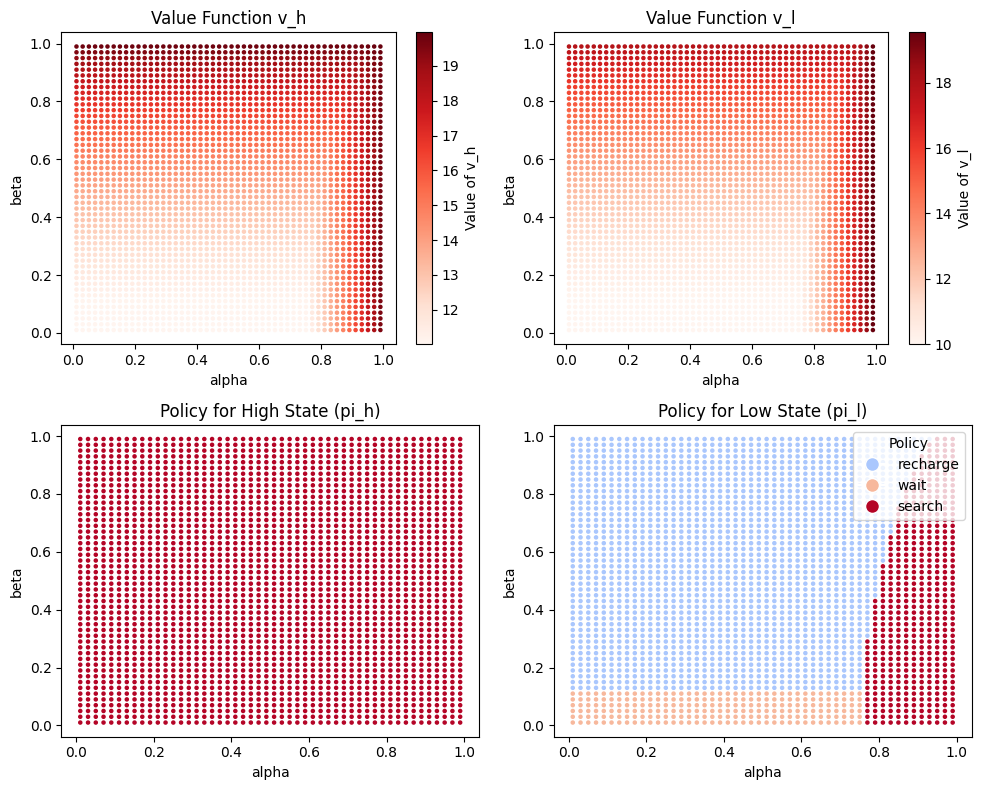
\includegraphics[width=\textwidth]{fig1.png} % Adjust the width as needed
    \caption{Results of the linear programming solution.}
    \label{fig:results}
\end{figure}

\begin{thebibliography}{99}

\bibitem{SuttonBarto2018} 
Sutton, R. S., \& Barto, A. G. (2018). \textit{Reinforcement learning: An introduction} (2nd ed.). MIT Press.


\bibitem{HelmertRoger2021}
Helmert, M., \& Röger, G. (2021). \textit{Planning and Optimization: F2. Bellman Equation \& Linear Programming}. Retrieved from \url{https://ai.dmi.unibas.ch/_files/teaching/hs21/po/slides/po-f02.pdf}

\end{thebibliography}

\end{document}
